\structure{ХОД РАБОТЫ}

В проекте был написан класс для решения рационального дележа в кооперативных играх.

Пример запуска программы:

\begin{codelisting}[language=Bash]
    go run cmd/lw5/main.go
\end{codelisting}

\section{Проверка на супераддитивность}

Игра является супераддитивной, если

\begin{equation}
\forall\, S,T \subseteq I \quad (S \cap T = \emptyset) \colon \ v(S \cup T) \geq v(S) + v(T).
\end{equation}

Данная игра является супераддитивной, так как для всех пар множеств выполняется условие (1).

\section{Проверка на выпуклость}

Игра является выпуклой, если

\begin{equation}
\forall S, T \subseteq I \colon v(S \cup T) + v(S \cap T) \geq v(S) + v(T).
\end{equation}

Данная игра не является выпуклой. Например, подставим $S = \{1, 2, 3\}$ и $T = \{1, 2, 4\}$ в формулу (2):

\begin{align*}
  v(\{1, 2, 3, 4\}) + v(\{1, 2\}) &\overset{?}{\geq} v(\{1, 2, 3\}) + v(\{1, 2, 4\}) \\
  14 + 6 &\overset{?}{\geq} 12 + 9 \\
  20 &< 21
\end{align*}

\section{Вектор Шепли}

Найдем вектор Шепли, элементы которого выражаются следующим выражением:

\begin{equation}
x_i(v) = \frac{1}{N!} \sum_{S \colon i \in S} (|S| - 1)! \, (N - |S|)! \, \big(v(S) - v(S \setminus \{i\})\big),
\end{equation}

С помощью программы посчитаем вектор Шепли:

\[
  X(v) = (3.25, 4.083, 4.75, 1.917)
\]

Проверим выполнение условия групповой рационализации, которое задается условием (4).

\begin{equation}
  \sum_{i \in I} x_i(v) = v(I)
\end{equation}

Для данной игры условие выполняется.

Проверим выполнение условия индивидуальной рационализации, которое задается условием (4).

\begin{equation}
  x_i(v) \geq v\bigl(\{i\}\bigr), \quad i \in I
\end{equation}

Для данной игры условие выполняется. Доказательство представлено на рисунке~\ref{fig:fig01}.

\begin{figure}
  \centering
  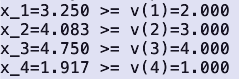
\includegraphics[scale=0.6]{../../artifacts/lw5/1.png}
  \caption{Проверка индивидуальной рационализации}
  \label{fig:fig01}
\end{figure}
